\documentclass[10pt]{article}
\title{Computer Science 2 - Assignment 2}
\author{Giacomo Ellero - 3243701}
\date{05/03/2024}

\usepackage{amsfonts}
\usepackage{amsthm}
\usepackage{amssymb}
\usepackage{amsmath}
\usepackage{mathtools}
\usepackage{commath}
\usepackage{dirtytalk}
\usepackage{parskip}
\usepackage{mathrsfs}
\usepackage[many]{tcolorbox}
\usepackage{xparse}
\usepackage[a4paper,margin=1.5cm]{geometry}
\usepackage{bookmark}
\usepackage{bytefield}
\usepackage{preamble_code}
\usepackage{capt-of}
\usepackage{tikz}
\usepackage{enumitem}
\usepackage{fancyhdr}
\usepackage{subfig}

\pagestyle{fancy}
\chead{Giacomo Ellero - 3243701}

\newcommand{\C}{\mathbb{C}}
\newcommand{\R}{\mathbb{R}}
\newcommand{\N}{\mathbb{N}}
\newcommand{\Z}{\mathbb{Z}}
\newcommand{\F}{\mathcal{F}}
\renewcommand{\Re}{\operatorname{Re}}
\renewcommand{\Im}{\operatorname{Im}}

\newenvironment{absolutelynopagebreak}
  {\par\nobreak\vfil\penalty0\vfilneg
   \vtop\bgroup}
  {\par\xdef\tpd{\the\prevdepth}\egroup
   \prevdepth=\tpd}

\newtcolorbox{examplebox}[1]{colback=green!5!white,colframe=green!40!black,title={#1},fonttitle=\bfseries,parbox=false}
\newtcolorbox{notebox}[1]{colback=blue!5!white,colframe=blue!40!black,title={Note: #1},fonttitle=\bfseries,parbox=false}
\newtcolorbox{bluebox}[1]{colback=blue!5!white,colframe=blue!40!black,title={#1},fonttitle=\bfseries,parbox=false}
\newtcolorbox{warningbox}[1]{colback=orange!5!white,colframe=orange!90!black,title={Warning: #1},fonttitle=\bfseries,parbox=false}
   
\begin{document}

\maketitle

\section*{Exercise 1}

\begin{enumerate}
    \item True. According to Kruskal's algorithm, the first edge to be added to the MST is the edge with the smallest weight, therefore $e$, being an edge of minimum weight, will be the first edge to be added to some MST, depending on the order in which the edges are considered.
    \item True. If we decrease the weight of $e$ it will still be the added to the MST, since it will still be the edge with the smallest weight. Moreover, since the cost of $T$ is the sum of the weights of the edges in $T$, the cost of $T$ will decrease because the weight of $e$ is part of the sum. Note that the fact that $c(e)$ decreased will not affect the other edges in $T$ because $e$ was going to be added to $T$ anyway.
    \item False. According to Kruskal's algorithm, we sort the list of edges by increasing weight and then we add the edges to the MST one by one as described by the algorithm. If the costs of the edges are not unique (i.e. $\exists, (u, v) \neq (u', v') \in E$ such that $C = c(u, v) = c(u', v')$), then it is possible that the MST is not unique because when get to the step where we add edges of cost $C$ the algorithm, in some cases, could choose to add $(u, v)$ instead of $(u', v')$ and vice versa. This is not always the case though, for example in the graph in Figure \ref{fig:counterexample_1} the MST is unique even though there are two edges of the same weight.

          \begin{figure}[H]
              \centering

              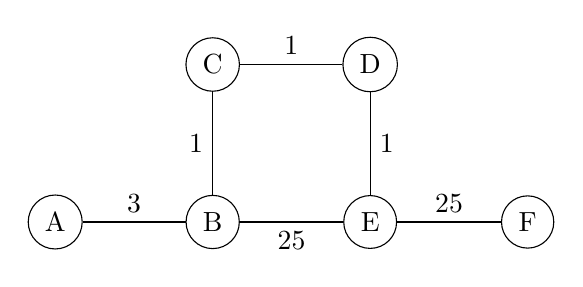
\begin{tikzpicture}
                  \node[draw, circle] (A) at (0, 0) {A};
                  \node[draw, circle] (B) at (2, 0) {B};
                  \node[draw, circle] (C) at (2, 2) {C};
                  \node[draw, circle] (D) at (4, 2) {D};
                  \node[draw, circle] (E) at (4, 0) {E};
                  \node[draw, circle] (F) at (6, 0) {F};


                  \draw (A) -- node[above] {3} (B);
                  \draw (B) -- node[left] {1} (C);
                  \draw (B) -- node[below] {25} (E);
                  \draw (C) -- node[above] {1} (D);
                  \draw (D) -- node[right] {1} (E);
                  \draw (E) -- node[above] {25} (F);

              \end{tikzpicture}

              \caption{Counterexample, a graph with two edges of the same weight that has a unique MST.}
              \label{fig:counterexample_1}
          \end{figure}

    \item False. We can use the graph in Figure \ref{fig:counterexample_2} as a counterexample. The idea of Dijkstra's algorithm is to find the shortest path from a source vertex to all the other vertices in the graph, not the best way to connect all vertices of the graph.
          Indeed the result that Dijkstra's algorithm gives depends on the choice of the start vertex, and in the counterexample provided below, starting from $S$ doesn't yield the MST.

          Note however that Dijkstra's algorithm can be modified into Prim's algorithm which is a similar algorithm which can be used to find the MST.
          \begin{figure}[H]
              \centering

              \subfloat[\centering Actual MST (green)]{{
                          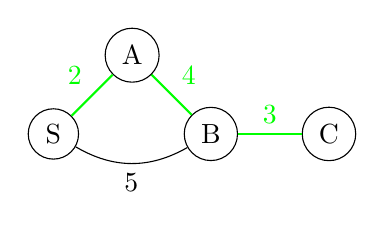
\begin{tikzpicture}
                              \node[draw, circle] (S) at (0, 0) {S};
                              \node[draw, circle] (A) at (1, 1) {A};
                              \node[draw, circle] (B) at (2, 0) {B};
                              \node[draw, circle] (C) at (3.5, 0) {C};


                              \draw[thick, green] (S) -- node[midway, anchor=south east] {2} (A);
                              \draw[thick, green] (A) -- node[midway, anchor=south west] {4} (B);
                              \draw[thick, green] (B) -- node[above] {3} (C);
                              \draw (S) to [bend right=30] node[below] {5} (B);
                          \end{tikzpicture}
                      }}\qquad
              \subfloat[\centering Dijkstra's choice (red)]{{
                          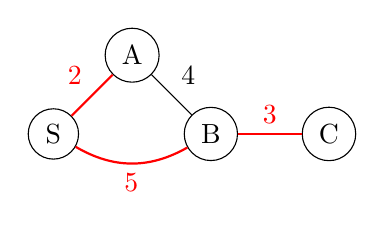
\begin{tikzpicture}
                              \node[draw, circle] (S) at (0, 0) {S};
                              \node[draw, circle] (A) at (1, 1) {A};
                              \node[draw, circle] (B) at (2, 0) {B};
                              \node[draw, circle] (C) at (3.5, 0) {C};


                              \draw[thick, red] (S) -- node[midway, anchor=south east] {2} (A);
                              \draw (A) -- node[midway, anchor=south west] {4} (B);
                              \draw[thick, red] (B) -- node[above] {3} (C);
                              \draw[thick, red] (S) to [bend right=30] node[below] {5} (B);
                          \end{tikzpicture}
                      }}
              \caption{Counterexample, a graph where Dijkstra's algorithm doesn't find the MST.}
              \label{fig:counterexample_2}
          \end{figure}
\end{enumerate}

\section*{Exercise 2}
\begin{enumerate}
    \item We can use the following algorithm to find the number of platforms needed:

          \begin{minted}{python}
def number_of_platforms(arrivals, departures):
    platforms = 0
    max_platforms = 0

    # Sort the arrival and departure times
    # from the earliest to the latest
    arrivals.sort()
    departures.sort()

    i = 0
    j = 0

    while i < len(arrivals) and j < len(departures):
        # If the earliest arrival is before the earliest departure
        # we need to add a platform, then we move to the next arrival
        if arrivals[i].is_before(departures[j]): 
            platforms += 1
            i += 1
        else:
            # Otherwise a train leaves, we can remove a platform
            # and check the next departure
            platforms -= 1
            j += 1

        # We keep track of the maximum number of platforms
        # we needed at each iteration
        max_platforms = max(max_platforms, platforms)
    
    return max_platforms
        \end{minted}

    \item
          We proceed by induction on the iterations of the \texttt{while} loop $t$ and we want to show that at each iteration \texttt{max\_platforms} is the maximum number of platforms needed at time $t$.

          \begin{description}
              \item[Base case] At $t = 0$ the number of platforms needed is indeed 0, and \texttt{max\_platforms} is also 0.
              \item[Induction step] Assuming that at time $t$ \texttt{max\_platforms} is the maximum number of platforms needed, we want to show that the same is true at $t + 1$.
                    Let $p_t$ be the number of platforms needed at time $t$.
                    Moreover, note that at $\texttt{max\_platforms} \geq p_t$ at the end of each iteration, because at each iteration we update \texttt{max\_platforms} to be the maximum of the current number of platforms and the previous maximum.

                    At each iteration we have the following cases:
                    \begin{enumerate}[label=\alph*)]
                        \item The next arrival is before the next departure, this means that the number of platforms $p_t$ is insufficient, therefore the algorithm will set $p_{t + 1} = p_t + 1$.
                        \item The next departure is before the next arrival, this means that the number of platforms we needed at $t$ is more than the trains in the station at $t+1$, therefore the algorithm can reduce it and set $p_{t + 1} = p_t - 1$.
                    \end{enumerate}

                    Now the algorithm will update \texttt{max\_platforms}.
                    Note that the maximum number of platforms needed at time $t + 1$ changes from what was needed at time $t$ only if we are in case a) and $p_{t + 1} > \texttt{max\_platforms}$. If the maximum number of platforms needed doesn't change the \texttt{max} function will keep the previous value, otherwise it will update it to $p_{t + 1}$.

                    Thus the invariant is preserved at each iteration.
          \end{description}

    \item The algorithm does the following operations:
          \begin{enumerate}[label=\alph*)]
              \item Sorts the arrival and departure times, which time complexity depends on the algorithm used but the most efficient comparison-based ones take $O(n \log n)$ time.
              \item Iterates through the arrival and departure times, which takes $O(n)$ time.
              \item Finding the maximum of two numbers takes $O(1)$ time.
          \end{enumerate}
          Therefore the time complexity of the algorithm is $O(n \log n)$.
\end{enumerate}

\end{document}